Residual networks address the degradation of accuracy of deep neural networks. Deep neural networks saturate, then degrade rapidly with increasing depth. Degradation is not caused by overfitting as increasing depth of suitably deep neural networks increases training error.\autocite{He.2016}
\blockquote[\cite{He.2016}]{
	The degradation (of training accuracy) indicates that not all systems are similarly easy to optimize. Let us consider a shallower architecture and its deeper counterpart that adds more layers onto it. There exists a solution by construction to the deeper model: the added layers are identity mappings, and the other layers are copied from the learned shallower model. The existence of this constructed solution indicates that a deeper model should produce no higher training error than its shallower counterpart.
}
Residual networks address the degradation problem by letting stacked layers learn the residual function $\mathcal{F}(X) = \mathcal{H}(X) - X$ instead of the desired function $\mathcal{H}(X)$. Thus, the original desired function is transformed into $\mathcal{F}(X) + X$. The shape of $\mathcal{F}(X)$ must match $X$. For differing shapes, $X$ is projected by $W$ to match shapes. This results in $\mathcal{F}(X) + WX$.
The formulation of $\mathcal{F}(X)+X$ can be implemented with shortcut connections. Shortcut connections are connections that skip one or more layers. A stack of layers that is skipped by a shortcut connection is called residual block, see Figure \ref{fig:resblock}.
This is based on the hypothesis that stacked layers can learn any function. This hypothesis is equivalent to the hypothesis that stacked layers can learn the residual functions $\mathcal{H}(X) - X$. \footnote{assuming that the input and output are of the same dimensions} Both approaches should be able to learn the desired functions. The difficulty of learning may vary.
Using residual networks, deeper neural networks can be learned. \autocite{He.2016}
\begin{figure}[H]
	\centering
	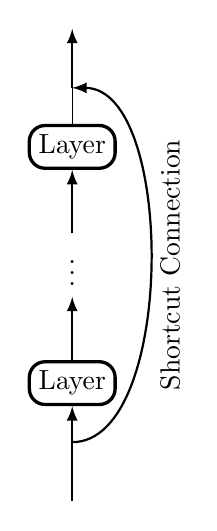
\begin{tikzpicture}[
	cell/.style={
		rectangle, 
		rounded corners=2mm, 
		draw,
		very thick,
		align=center,
	},
	ArrowC1/.style={% Arrows with rounded corners
		rounded corners=.25cm,
		thick,
	},
]
	\coordinate (out) at (0,6);
	\coordinate (inbranch) at (0,5.25);
	\node [cell] (ln) at (0,4.5) {Layer};
	\node [very thick, align = center](dots) at (0,3) {\vdots};
	\node [cell] (l1) at (0,1.5) {Layer};
	\coordinate (outbranch) at (0,0.75);
	\coordinate (in) at (0,0);
	
	\draw [-latex,ArrowC1] (inbranch) -- (out);
	\draw (ln) -- (inbranch);
	\draw [-latex,ArrowC1] (dots) -- (ln);
	\draw [-latex,ArrowC1] (l1) -- (dots);
	\draw [-latex,ArrowC1] (outbranch) -- (l1);
	\draw [thick] (in) -- (outbranch);
	
	\draw [-latex,ArrowC1,out=0,in=0,looseness=0.75] (outbranch) to node[sloped,below]{Shortcut Connection}  (inbranch);
\end{tikzpicture}
	\caption{Residual Block (own figure)} \label{fig:resblock}
\end{figure}
\par
The best-performing residual network found in the course of the literature review is the $152$-layer version of \cite{He.2016}'s ResNet, called ResNet-152.
The input of ResNet-152 is a $224$-by-$224$-pixel, \ac{RGB} image. The output of ResNet-152 comprises the probabilities of the $c$~target classes. \autocite{He.2016}
\par
ResNet-152 is comprised of $151$ convolutional layers followed by $1$ dense layer.
The convolutional layers have a stride of $1$, unless specified otherwise.
The convolutional layers use batch normalization and the \ac{ReLU} activation function.
Batch normalization is applied after every convolution before the activation function.
The dense layer has $c$ neurons and uses the softmax activation function.
The first convolutional layer is followed by max pooling, has a kernel size of $7$, and a stride of $2$.
Max pooling is applied with a pooling size of $3$ and a pooling stride of $2$. \autocite{He.2016}
\par
The remaining covolutional layers are arranged in residual blocks. A residual block consists of three stacked convolutional layers and a shortcut connection. The first and third layer have a kernel size of $1$. The second layer has a kernel size of $3$. The first and third layer are used to reduce, then increase (restore) dimensions. This way, the second layer becomes a bottleneck with smaller input/output dimensions. On that account, computation costs are reduced.
The shortcut connection skips the three layers. The shortcut connection uses identity mapping. The output of the identity mapping is added element-wise to the output of the skipped layers. The result transformed by the \ac{ReLU} activation function is the output of the block.
ResNet-152 consists of 4 types of stacked blocks. The types differ only in the number of kernels of their layers. The configurations of each residual block are outlined in Table \ref{tab:resnet}. \autocite{He.2016} 
\par
The first layer of the first block of a type has a stride of $2$. This way, the feature map size is halved while the number of filters is doubled. Hence, the time complexity per layer is preserved.
The last layer of the last block is followed by global average pooling. \autocite{He.2016}
\par
The whole configuration of ResNet-152 is outlined in Table \ref{tab:resnet}. \autocite{He.2016}
\begin{xltabular}{\textwidth}{lX}\toprule
	\caption[ResNet-152 Configuration]{ResNet-152 Configuration. Note that each $k \times k \text{ conv } K$ denotes a convolutional layer with $K$ kernels of size  $k$. A residual block is denoted as an array of layers.} \label{tab:resnet}\\
	\textbf{Layer/Block} & \textbf{Configuration}\\\midrule \endhead
	Input Layer & $7 \times 7 \text{ conv } 64$, stride $2$, and $3 \times 3$ max pooling, stride $2$\\\midrule
	Residual Block $1-3$ & $\begin{bmatrix}
	1 \times 1 \text{ conv } 64\\
	3 \times 3 \text{ conv } 64\\
	1 \times 1 \text{ conv } 256
	\end{bmatrix} \times 3$\\\midrule
	Residual Block $4-11$ & $\begin{bmatrix}
	1 \times 1 \text{ conv } 128\\
	3 \times 3 \text{ conv } 128\\
	1 \times 1 \text{ conv } 512
	\end{bmatrix} \times 8$\\\midrule
	Residual Block $12-47$ & $\begin{bmatrix}
	1 \times 1 \text{ conv } 256\\
	3 \times 3 \text{ conv } 256\\
	1 \times 1 \text{ conv } 1024
	\end{bmatrix} \times 36$\\\midrule
	Residual Block $48-50$ & $\begin{bmatrix}
	1 \times 1 \text{ conv } 512\\
	3 \times 3\text{ conv } 512\\
	1 \times 1\text{ conv } 2048
	\end{bmatrix} \times 3$\\\midrule
	Output Layer & global average pooling, dense with $c$ neurons
	\\\bottomrule
\end{xltabular}